\documentclass[tikz]{standalone}

\usepackage{fontspec}

\usetikzlibrary{arrows}
\usetikzlibrary{calc}
\usetikzlibrary{decorations.pathreplacing}
\usetikzlibrary{positioning}
\usetikzlibrary{matrix}

\begin{document}

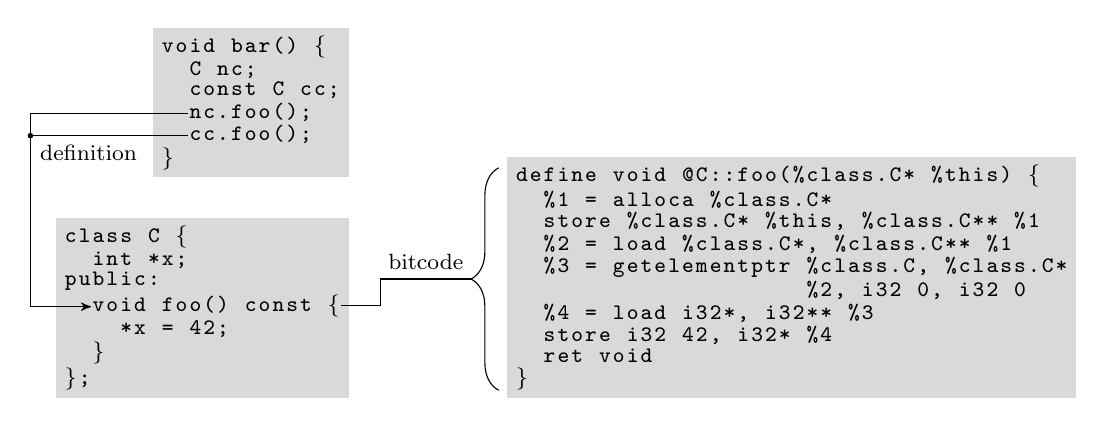
\begin{tikzpicture}
  [node distance=5mm, >=stealth',
  every node/.style={font=\footnotesize},
  every matrix/.style={fill=black!15, inner sep=1mm, row sep=0.5mm,
                        matrix of nodes, nodes in empty cells, minimum width=.5em,
                        nodes={anchor=base, inner sep=0, font=\ttfamily\footnotesize}}]

  \matrix (bar) {
v & o & i & d &   & b & a & r & ( & ) &   & \{ &   \\

  &   & C &   & n & c & ; &   &   &   &   &   &   \\

  &   & c & o & n & s & t &   & C &   & c & c & ; \\

  &   & n & c & . & f & o & o & ( & ) & ; &   &   \\

  &   & c & c & . & f & o & o & ( & ) & ; &   &   \\

\} &   &   &   &   &   &   &   &   &   &   &   &   \\
  };

  \matrix (C) [below=of bar.south east, anchor=north east]
  {
c & l & a & s & s &   & C &   & \{ &   &   &   &   &   &   &   &   &   &   &   \\

  &   & i & n & t &   & * & x & ; &   &   &   &   &   &   &   &   &   &   &   \\


p & u & b & l & i & c & : &   &   &   &   &   &   &   &   &   &   &   &   &   \\

  &   & v & o & i & d &   & f & o & o & ( & ) &   & c & o & n & s & t &   & \{ \\

  &   &   &   & * & x &   & = &   & 4 & 2 & ; &   &   &   &   &   &   &   &   \\

  &   & \} &   &   &   &   &   &   &   &   &   &   &   &   &   &   &   &   &   \\

\} & ; &   &   &   &   &   &   &   &   &   &   &   &   &   &   &   &   &   &   \\
  };

  \matrix (bitcode) [node distance=2cm, right=of C.south east, anchor=south west] {
d & e & f & i & n & e &   & v & o & i & d &   & @ & C & : & : & f & o & o & ( & \% & c & l & a & s & s & . & C & * &   & \% & t & h & i & s & ) &   & \{ &   &   \\

  &   & \% & 1 &   & = &   & a & l & l & o & c & a &   & \% & c & l & a & s & s & . & C & * &   &   &   &   &   &   &   &   &   &   &   &   &   &   &   &   &   \\

  &   & s & t & o & r & e &   & \% & c & l & a & s & s & . & C & * &   & \% & t & h & i & s & , &   & \% & c & l & a & s & s & . & C & * & * &   & \% & 1 &   &   \\

  &   & \% & 2 &   & = &   & l & o & a & d &   & \% & c & l & a & s & s & . & C & * & , &   & \% & c & l & a & s & s & . & C & * & * &   & \% & 1 &   &   &   &   \\

  &   & \% & 3 &   & = &   & g & e & t & e & l & e & m & e & n & t & p & t & r &   & \% & c & l & a & s & s & . & C & , &   & \% & c & l & a & s & s & . & C & * \\

  &   &   &   &   &   &   &   &   &   &   &   &   &   &   &   &   &   &   &   &   & \% & 2 & , &   & i & 3 & 2 &   & 0 & , &   & i & 3 & 2 &   & 0 &   &   &   \\

  &   & \% & 4 &   & = &   & l & o & a & d &   & i & 3 & 2 & * & , &   & i & 3 & 2 & * & * &   & \% & 3 &   &   &   &   &   &   &   &   &   &   &   &   &   &   \\

  &   & s & t & o & r & e &   & i & 3 & 2 &   & 4 & 2 & , &   & i & 3 & 2 & * &   & \% & 4 &   &   &   &   &   &   &   &   &   &   &   &   &   &   &   &   &   \\

  &   & r & e & t &   & v & o & i & d &   &   &   &   &   &   &   &   &   &   &   &   &   &   &   &   &   &   &   &   &   &   &   &   &   &   &   &   &   &   \\

\} &   &   &   &   &   &   &   &   &   &   &   &   &   &   &   &   &   &   &   &   &   &   &   &   &   &   &   &   &   &   &   &   &   &   &   &   &   &   &   \\
};

  \draw let \p1 = (bar-4-3.west),
            \p2 = (bar-5-3.west)
        in (\p1) -- (\x1 - 2cm, \y1) -- (\x1 - 2cm, \y2);

  \fill ($ (bar-5-3.west) - (2cm,0) $) circle (1pt)
        node [below right] {definition};

  \draw[->] let \p1 = (bar-5-3.west),
                \p2 = (C-4-3.west)
            in (\p1) -- (\x1 - 2cm, \y1) -- (\x1 - 2cm, \y2) -- (\x2, \y2);

  \draw[decorate, decoration={brace, amplitude=10pt, mirror}]
       ($ (bitcode-1-1.north west) - (2mm, 0) $)
       -- ($ (bitcode-10-1.south west) - (2mm, 0) $);

  \draw let \p1 = ($ (bitcode-10-1.south west)!0.5!(bitcode-1-1.north west)
                     - (2mm + 10pt,0) $),
            \p2 = (C-4-20.east)
        in (\p2) -- (\x2 + 5mm, \y2) -- (\x2 + 5mm, \y1)
        -- node [above] {bitcode} (\p1);

\end{tikzpicture}

\end{document}
